\chapter{The Experiment} \label{chap:chap-3}


% epigraph after chapter heading
\epigraph{We are experimentalists.}{-- Andrei Gritsan}


%%%% MUST: add the citation for the chapter if it is a reprint



%% remove the following and add your chapter text here
\section{The Large Hadron Collider}


Since its first start-up on 10 September 2008, the Large Hadron Collider (LHC) has been the world’s largest and most energetic particle accelerator. It is so named because it is very large, consisting of a 27 km ring of superconducting magnets; accelerates hadrons, usually protons or ions; and collides these particles via two beams travelling in opposite directions, which intersect at four points along the circuference of the machine.

\begin{figure}[!ht]
    \begin{center}
        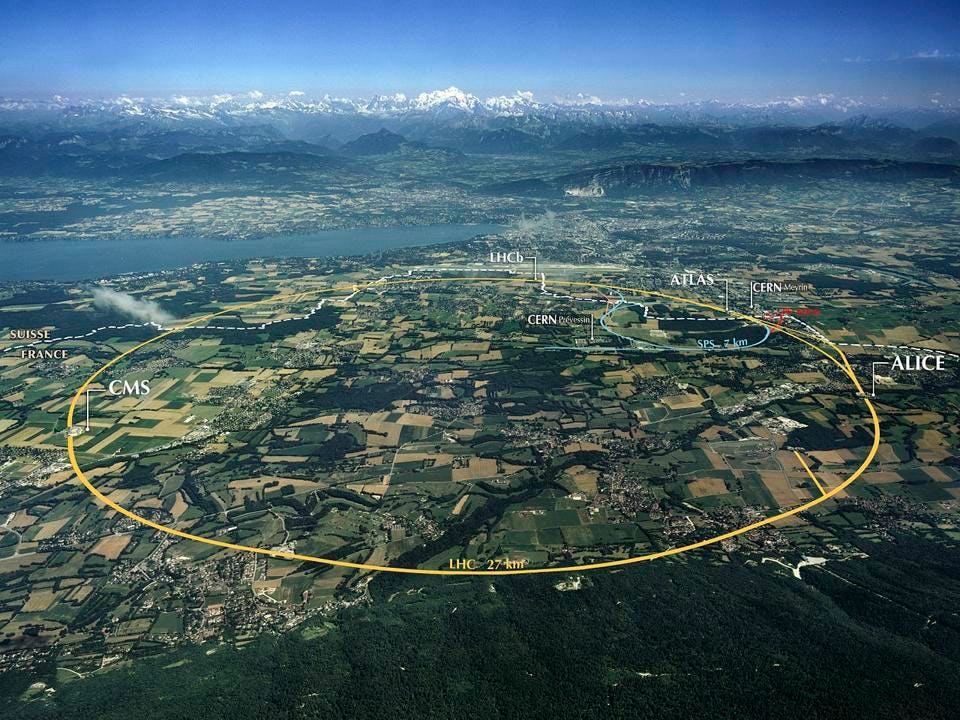
\includegraphics[width=0.8\textwidth,clip] {LHCaerial.jpg}
        \caption{An aerial view of CERN.}
        \label{fig:LHCaerial}
    \end{center}
    \end{figure}

The size of any accelerator is related to the maximum energy it can acheive. 
In the case of the LHC, this energy is proportional to the radius of the
machine and the strength of the magnetic fields that keep the accelerating particles stable. 
The LHC re-uses the 27 km circumference tunnel that was built for the previous big accelerator, the Large Electron-Positron Collider (LEP), which was dismantled in 2000.
The underground tunnel was the best solution to house a 27-km circumference machine because it was cheaper to excavate a tunnel rather than acquire the land to build at the surface.
In addition, the Earth’s crust provides good shielding for radiation. 
As such, the dimensions of the tunnel and capabilities of the magnets, cavities and other essential elements enforce the primary constraints which determine our design energy of 7 TeV per proton beam \cite{CERNBroc79}. 

The tunnel was built at a mean depth of 100 m, due to geological considerations (again translating into cost) and at a slight gradient of 1.4\%. 
Its depth varies between 175 m (under the Jura) and 50 m (towards Lake Geneva), as the LHC crosses the French-Swiss border.

\begin{table}[]
    \centering
    \begin{tabular}{|l|l|}
    \hline
    Design Parameter                & Value                                                                           \\ \hline
    Circumference                   & 26659 m                                                                        \\
    Dipole operating temperature    & 1.9 K (-271.3 ºC)                                                               \\
    Number of magnets               & 9593                                                                            \\
    Number of main dipoles          & 1232                                                                            \\
    Number of main quadrupoles      & 392                                                                             \\
    Number of RF cavities           & 8 per direction                                                                 \\
    Energy, protons                 & 7 TeV                                                                           \\
    Energy, ions                    & 2.76 TeV/u                                                                      \\
    Peak magnetic dipole field      & 8.3 T                                                                           \\
    Distance between bunches        & $\sim$7.5 m                                                                     \\
    Luminosity (protons)            & $10^{34} cm^{-2} s^{-1}$ \\
    No. of bunches per proton beam  & 2808                                                                            \\
    No. of protons per bunch        & 1.1 x 1011                                                                      \\
    Number of turns per second      & 11245                                                                           \\
    Number of collisions per second & 1 billion                                                                       \\ \hline
    \end{tabular}
    \caption{Design parameters for the LHC}
    \label{tab:LHCparam}
\end{table}

Superconducting electromagnets are specifically designed to generate a powerful magnetic field of 8.3 T around the circumference of the collider. LHC dipoles use niobium–titanium (NbTi) cables, which become superconducting below a temperature about 10 K (-263.2 °C)\footnote{The LHC actually operates at 1.9 K (-271.3 °C) and the beam pipes are kept at ultrahigh vacuum ($10^{-10}$ to $10^{-11}$ mbar), even colder than outer space (2.7 K or -270.5 °C) and close to the atmospheric pressure of the Moon's surface!}. Approximately 10000 superconducting magnets are installed in the LHC. Among these, 1232 dipole magnets, each 15 meters long, guide the beam around the accelerator ring, while 392 quadrupole magnets, each measuring between 5 and 7 meters, focus the beam. Additional stronger quadrupole magnets are positioned near interaction points\footnote{Just prior to collision, magnets will squeeze the particles closer together to increase the chances of collisions. The incoming particles are so small that the task of ensuring collision is akin to firing two needles 10 km apart with such precision that they meet halfway.}, along with multipole magnets to fine-tune the beam and refocus it after any deflection. The beam particles' energy is boosted by 0.5 MeV per turn using 16 radiofrequency (RF) cavities. To maintain the superconducting magnets at their operating temperature of 1.9K (-271.3°C), 96 tonnes of liquid helium is used. 

All the controls for the accelerator, its services, and technical infrastructure are housed under one roof at the CERN Control Centre. From here, the beams inside the LHC are steered to collide at four locations around the accelerator ring, corresponding to the positions of four particle detectors -- ATLAS, CMS, ALICE, and LHCb. Of these, CMS and ATLAS are general purpose detectors, while LHCb is sensitive to the physics of b quarks, and ALICE studies quark-gluon plasmas utilizing heavy-ion collisions.

The protons of the LHC circulate around the ring in well-defined bunches -- a direct consequence of the radio frequency (RF) acceleration scheme. 
Under nominal operating conditions, each proton beam has 2808 bunches, with each bunch containing about $10^{11}$ protons. 
The particles in these bunches are so small that the probability of any two colliding is very low. When the bunches cross at a colision point, there are up to 40 collisions between the total 200 billion particles. Bunches cross on average about 30 million times per second, so the LHC generates about 1 billion particle collisions per second.

This gives us our total design luminosity, which is the total number of proton-proton interactions. However, when studying a particular physics process, the probability of the process to occur in a given interaction is given by a factor which we call cross-section ($\sigma$). Thus the number of events per second created at the LHC for a certain physics process is calculated as:

\begin{equation}
\label{eq:crosssection}
\begin{gathered}
\frac{dN}{dt} = \mathcal{L} \times \sigma.
\end{gathered}
\end{equation}



\section{The Central Muon Solenoid}
The Central Muon Solenoid (CMS) detector is built around a large superconducting solenoid, for which it is named. It spans 6 meters in its internal diameter and generates a magnetic field of 3.8 Tesla. This very large field bends the trajectories of charged particles which helps to identify their momenta along with charge information. Inside the solenoid we find silicon trackers and calorimeters, while outside the solenoid we have layers of muon detection chambers.

\begin{figure}[!ht]
\begin{center}
    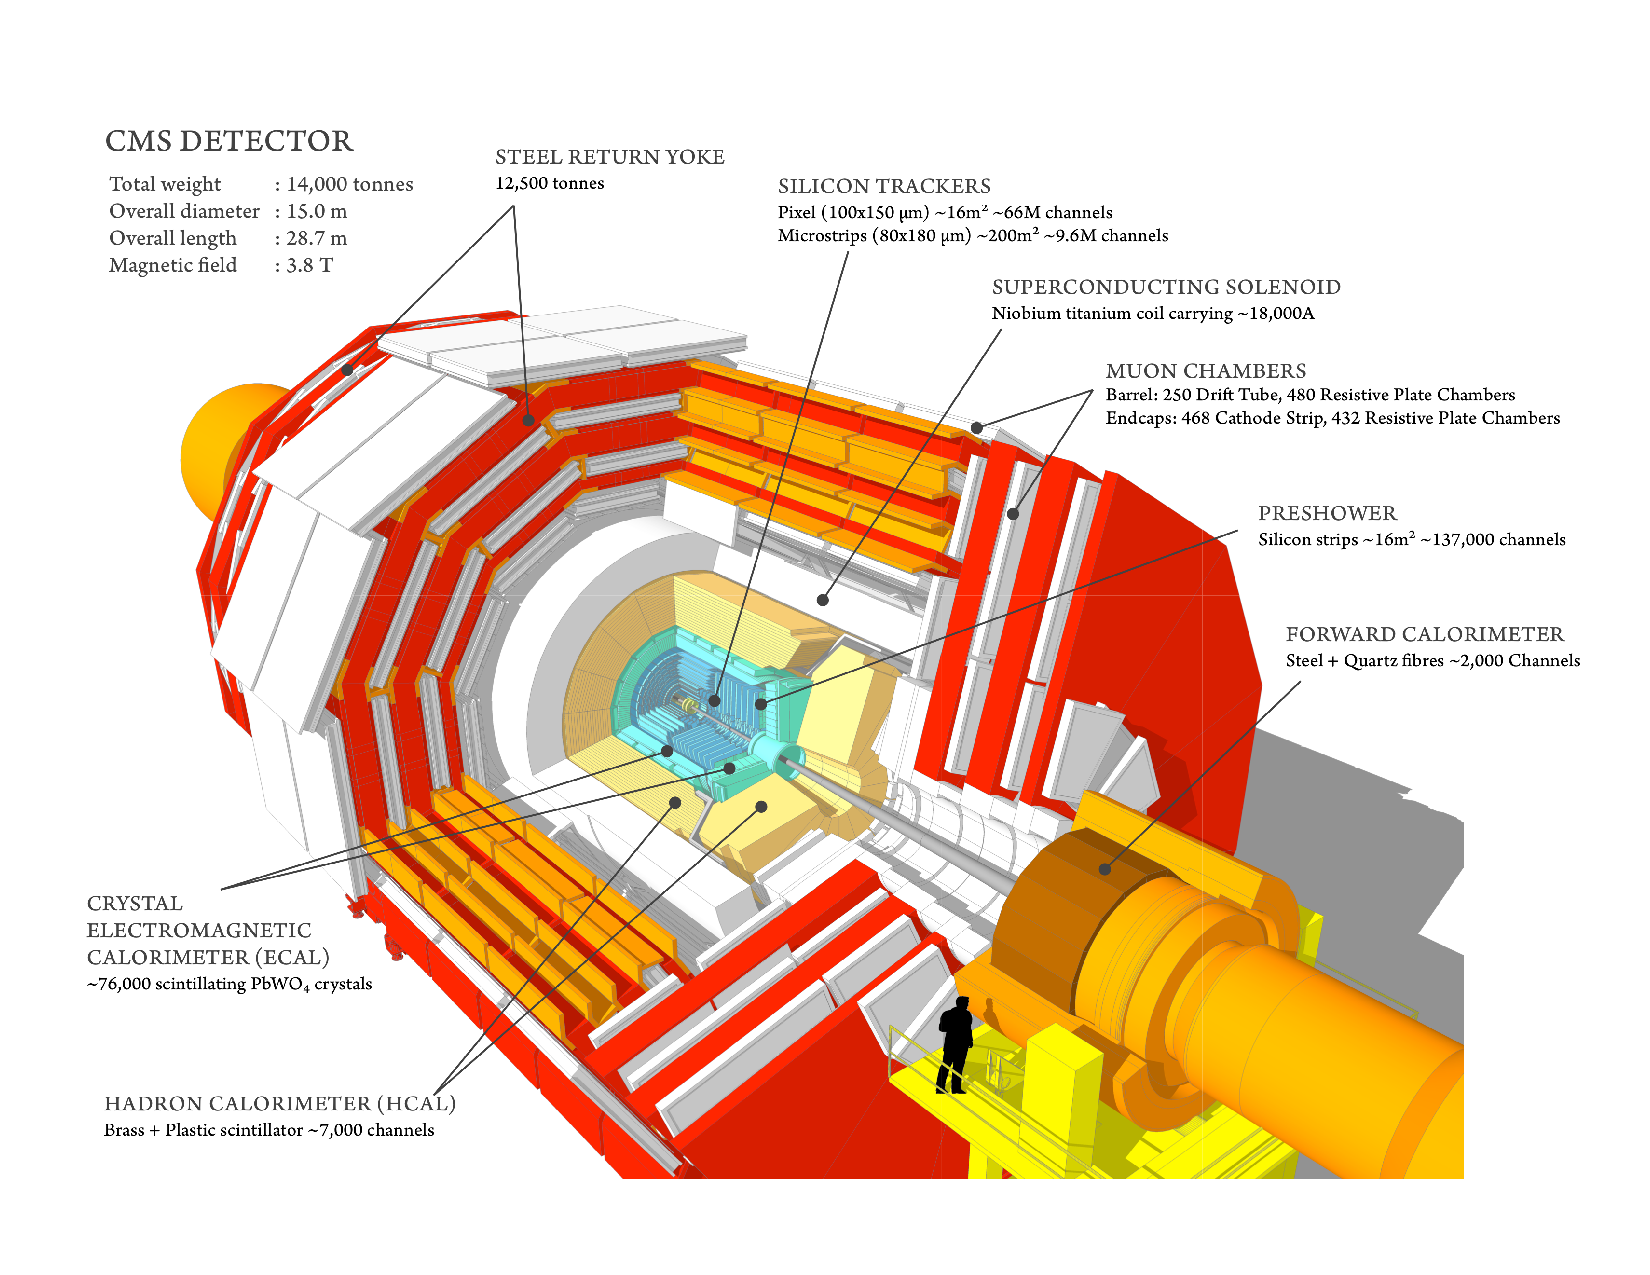
\includegraphics[width=0.8\textwidth,clip] {cmsdetector.pdf}
    \caption{The CMS detector is shaped like a cylindrical onion, with several concentric layers of components \cite{CMS}.}
    \label{fig:cmscutaway1}
\end{center}
\end{figure}

CMS in effect acts like a high-speed camera, taking 3-dimensional ``snapshots'' of particle collision events in all directions up to 40 million times each second. Although most of the initial collision products decay rapidly, the stable particles which they spawn can be detected by CMS. By identifying the stable particles produced in each collision and then piecing them together, the detector can recreate a picture of the collision which can then be analyzed to identify constituent physics phenomena \cite{Karimaki:368412, CERN-LHCC-2000-016, Chatrchyan:1129810, Collaboration:2745805, CERN-LHCC-2017-009}.

\subsection{Solenoid}
The superconducting solenoid is pivotal to the construction and operation of CMS, and has a 6 m internal diameter.
This magnet is the largest superconducting magnet ever built, weighing in at 12000 tonnes, and is cooled to -268.5ºC, almost as cold as outer space. 
The magnetic field of 3.8 T it generates is 100,000 times stronger than the Earth’s own magnetic field.

This large field is used to bend the paths of particles emerging from our high-energy collisions. Particles with more momentum have trajectories less affected by the magnetic field, so with high-precision position measurements from our tracking system and a precise tuning of such a strong magnetic field, we can make accurate measurements of the momentum of even high-energy particles. 

As previously mentioned, the tracker and calorimeter detectors (ECAL and HCAL) fit inside the magnet coil while the muon detectors are interleaved with a 12-sided iron structure that surrounds the magnet coils and contains and guides the field. Made up of three layers this structure, referred to as the ``return yoke,'' reaches out 14 m in diameter and also acts as a physical filter, through which only muons and weakly interacting particles such as neutrinos can traverse. The enormous solenoid also provides most of the experiment’s structural support, and is very robust to withstand the forces of its own magnetic field.

\begin{figure}[!ht]
    \begin{center}
        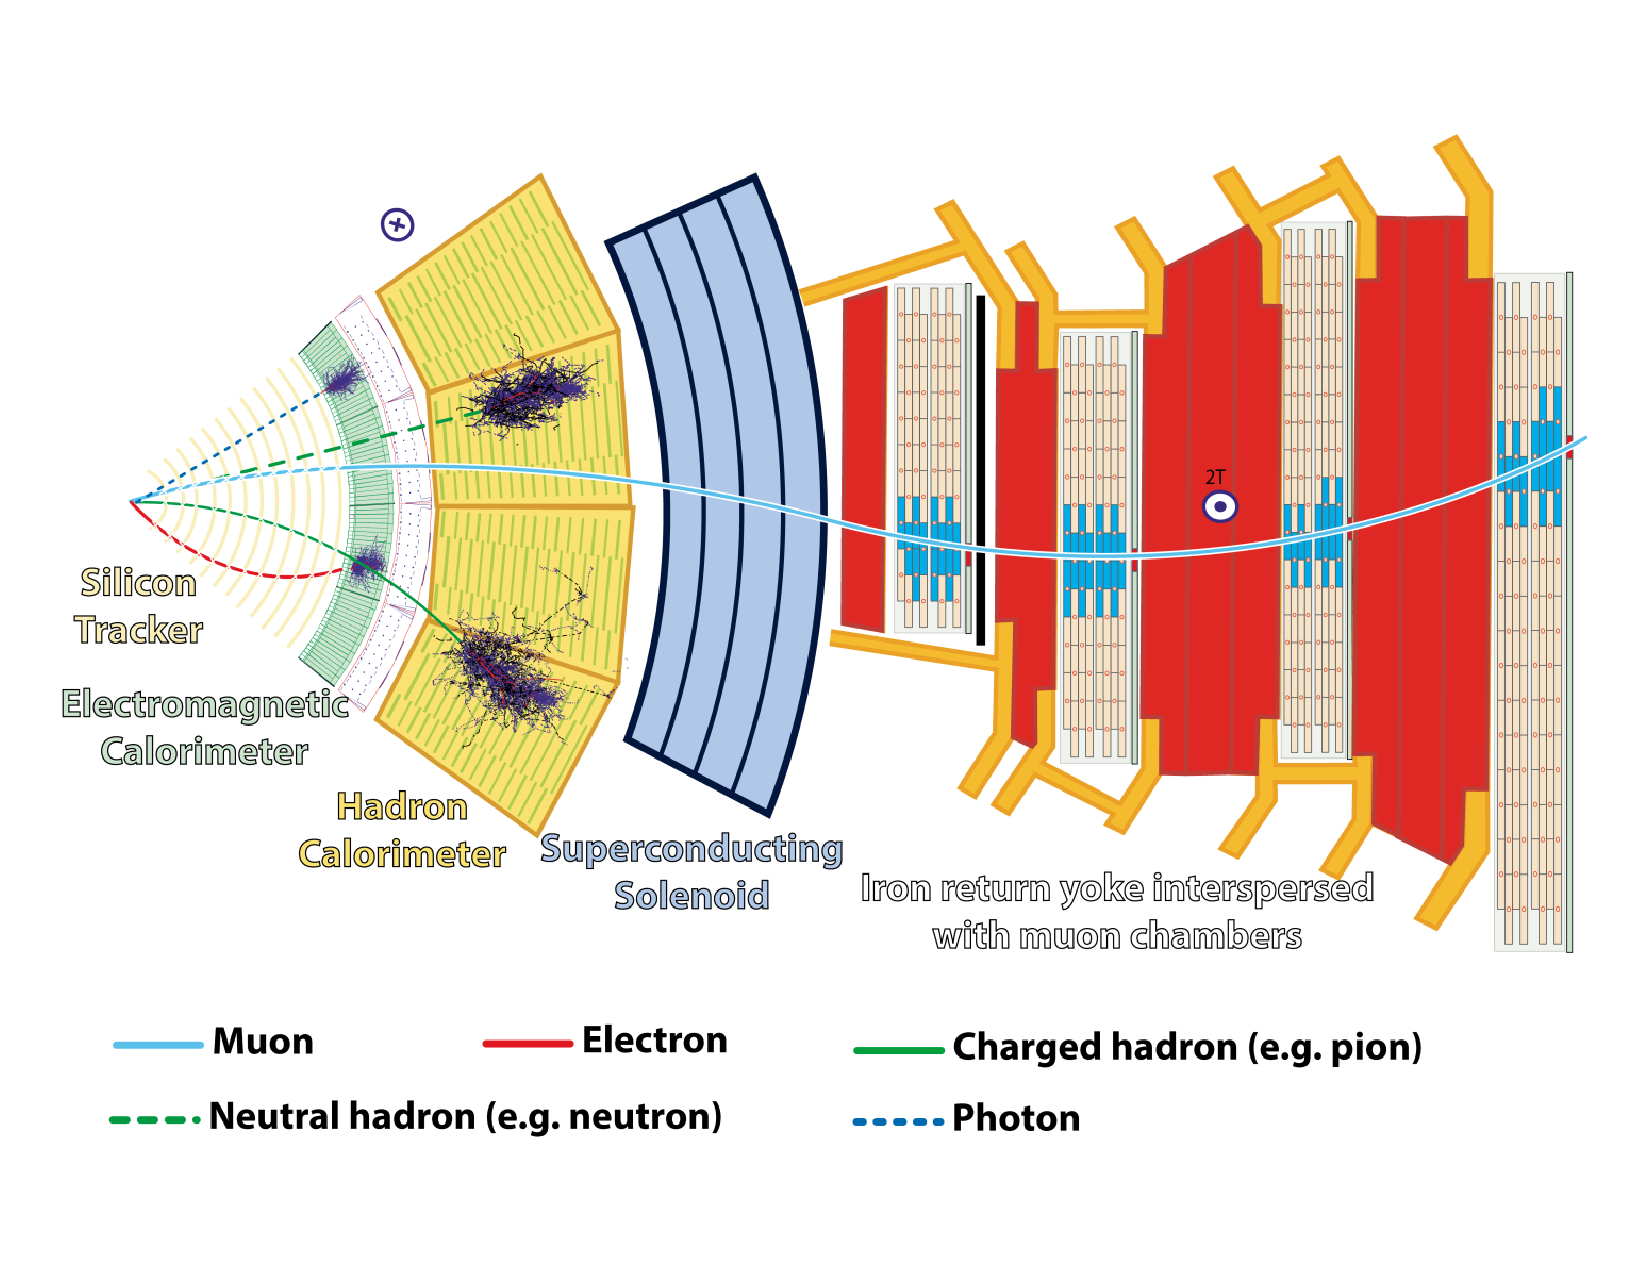
\includegraphics[width=0.8\textwidth,clip] {CMSslice.pdf}
        \caption{Schematic view of CMS detector \cite{CMS}.}
        \label{fig:cmscutaway2}
    \end{center}
\end{figure}

\begin{figure}[!ht]
    \begin{center}
        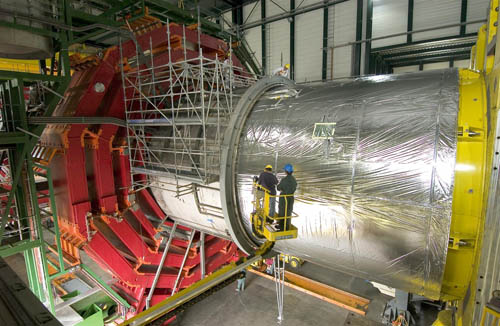
\includegraphics[width=0.8\textwidth,clip] {CMSmagnet.jpg}
        \caption{View of the CMS magnet during construction.}
        \label{fig:CMSmagnet}
    \end{center}
\end{figure}

\subsection{Silicon Tracker}

\begin{figure}[!ht]
    \begin{center}
        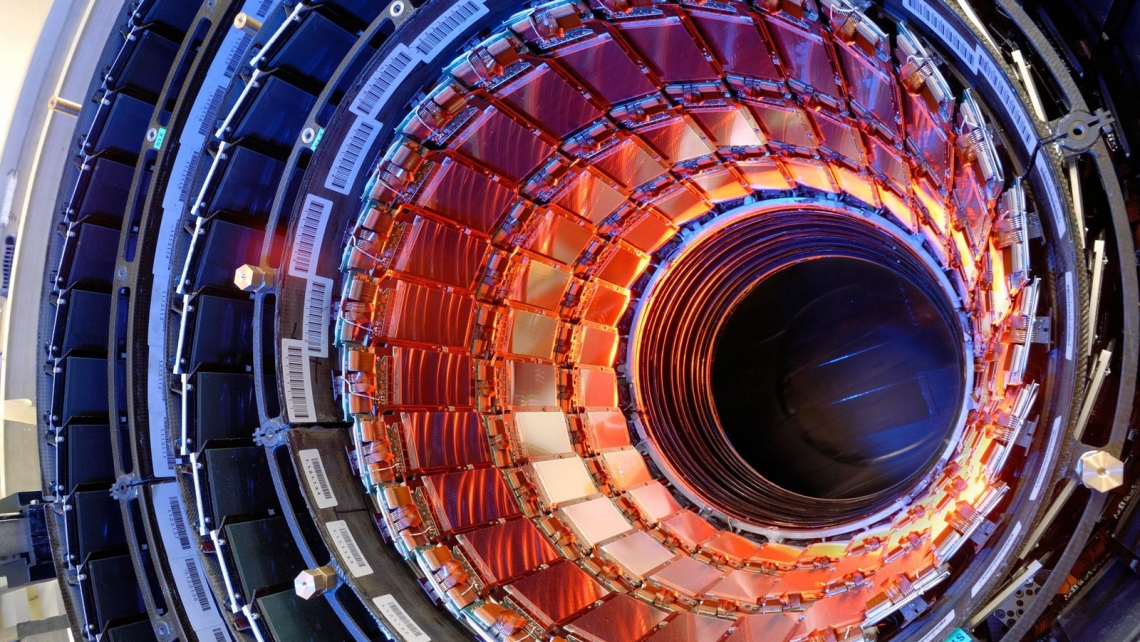
\includegraphics[width=0.8\textwidth,clip] {CMStracker.jpg}
        \caption{CMS Tracker showing silicon strips detectors in the barrel module.}
        \label{fig:CMStracker}
    \end{center}
\end{figure}

The tracker must precisely record particle paths while remaining lightweight to minimize interference with the particles. 
It achieves this by capturing highly accurate position measurements, allowing tracks to be reliably reconstructed with only a few data points. 
Each measurement has an accuracy of 10 µm, which is a fraction of the width of a human hair. 
As the innermost component of the CMS detector, the tracker is exposed to the highest volume of particles, so its construction materials were carefully selected for radiation resistance.

The tracker is assembled from several distinct detector elements, consisting of two silicon pixel subdetectors, the Tracker Pixel Barrel (TPB) and Tracker Pixel Endcap (TPE); 
and four silicon strip subdetectors, the Tracker Outer Barrel (TOB), Tracker Inner Barrel (TIB), Tracker Inner Disks (TID), and Tracker Endcap (TEC) \cite{Chatrchyan:1667597}.

\begin{figure}[!ht]
    \begin{center}
        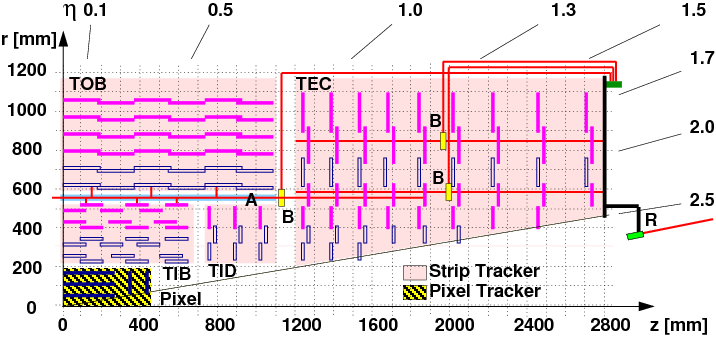
\includegraphics[width=0.8\textwidth,clip] {TrackerLayoutWithLAS.png}
        \caption{Schematic view of one quarter of the silicon tracker in the r-z plane.}
        \label{fig:CMStracker}
    \end{center}
\end{figure}


\subsubsection{Pixel Detector}

\begin{figure}[!ht]
    \begin{center}
        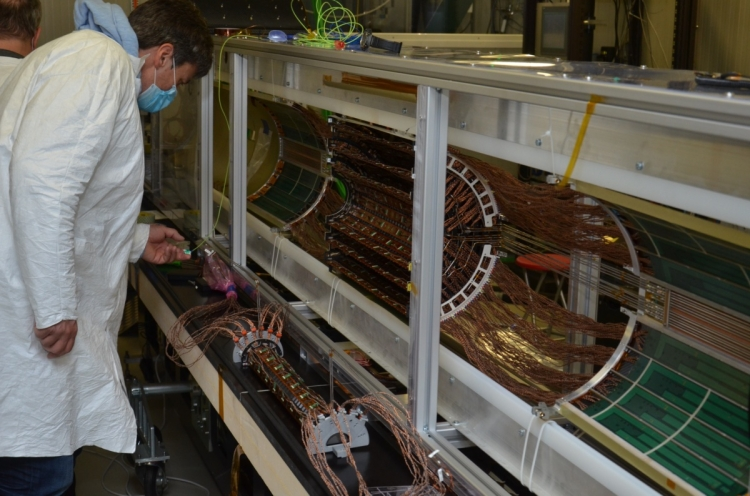
\includegraphics[width=0.8\textwidth,clip] {CMSpixel.jpg}
        \caption{Silicon pixel detector before installation.}
        \label{fig:CMSpixel}
    \end{center}
\end{figure}

\begin{figure}[!ht]
    \begin{center}
        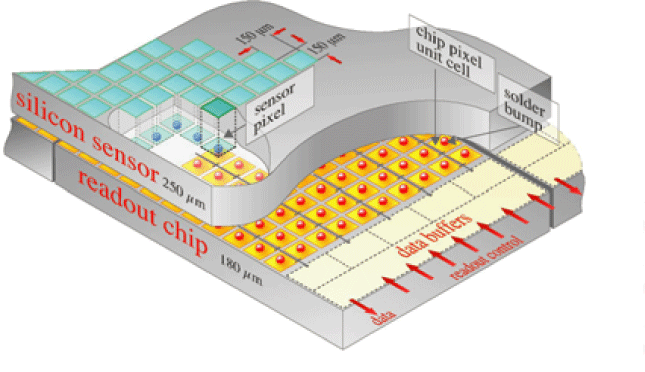
\includegraphics[width=0.8\textwidth,clip] {Pixelement.png}
        \caption{CMS silicon pixel detector.}
        \label{fig:CMSpixel}
    \end{center}
\end{figure}

The pixel detector, despite being only about the size of a shoebox, contains 124 million pixels, enabling it to track particle paths with exceptional accuracy as they emerge from collisions. 
Positioned closest to the beam pipe, it features cylindrical layers located approximately at radii of 3 cm, 7 cm, 11 cm, and 16 cm, with disks at either end. 
This proximity makes the pixel detector crucial for reconstructing the tracks of very short-lived particles.

Each of the four layers is composed of individual silicon modules, split into numerous pixels. Each of these silicon pixels is 100µm by 150µm, about the width of two human hairs. 
When a charged particle passes through a pixel, it ejects electrons from the silicon atoms. A voltage applied to the sensor allows the collection of these charges as a small electric signal, which is then amplified by an electronic readout chip (with a total of 16 chips per module). This design allows for significant bandwidth from the pixel detector, which is necessitated by the proximity to the point of collisions. The rate of particles received at 3 cm from the beamline is around 600 million particles per square centimeter per second.

Knowing which pixels have been energized allows us to deduce the particle's trajectory. And because the detector has 124 million of these pixels, arranged in four stacked layers of silicon modules, we can create a three-dimensional picture of each particle's path.


\subsubsection{Strip Detector}

\begin{figure}[!ht]
    \begin{center}
        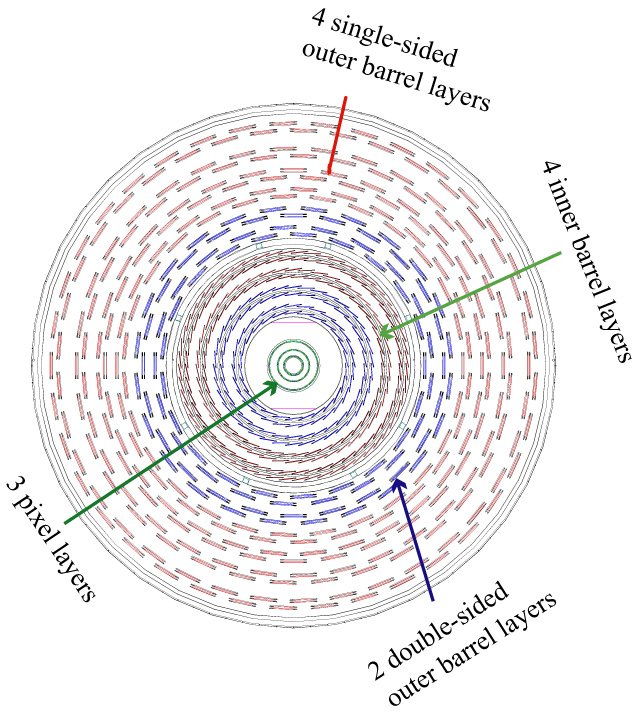
\includegraphics[width=0.8\textwidth,clip] {CMSBarrel.png}
        \caption{CMS Tracker layers shown in the plane perpendicular to the beam.}
        \label{fig:CMSBarrel}
    \end{center}
\end{figure}

After traversing the pixel detectors, particles move through ten layers of silicon strip detectors, which extend to a radius of 130 centimeters.

The silicon strip detector is composed of four inner barrel (TIB) layers and two inner endcaps (TID), each made up of three small discs. Surrounding both the TIB and TID is the outer barrel (TOB), consisting of six concentric layers. At either end of the tracker, two endcaps (TEC) provide closure. Each of these components contains silicon modules, wtih geometries optimized for their specific location within the detector.

This section of the tracker contains 15,200 highly sensitive modules, with a total of approximately 10 million detector strips read by 72,000 microelectronic chips. Each module comprises three main elements: one or two silicon sensors, a mechanical support structure, and readout electronics.

\subsection{Electromagnetic Calorimeter}

The Electromagnetic Calorimeter (ECAL) is the inner layer of the two calorimeters and measures the energy of electrons and photons by stopping them completely. 

\begin{figure}[!htb]
    \begin{center}
        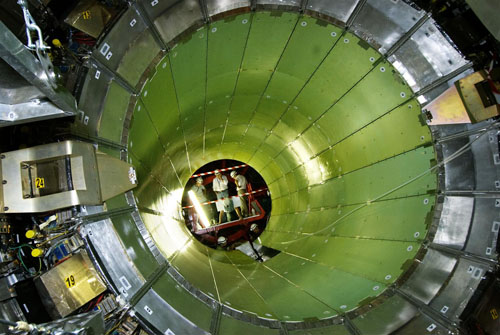
\includegraphics[width=0.8\textwidth,clip] {ECAL.jpg}
        \caption{CMS ECAL during construction.}
        \label{fig:ECAL}
    \end{center}
\end{figure}

The ECAL is constructed using nearly 80000 lead tungstate crystals, which are made primarily of metal (bound with oxygen in this crystalline form) and each weigh 1.5 kg. These crystals are incredibly dense yet highly transparent, and scintillate when electrons and photons pass through them. The light is produced in short, well-defined photon bursts which allows for precise identifications of the passing charged particles.

\subsection{Hadron Calorimeter}

Hadrons, which are composite particles made up of quarks and gluons, fly through the ECAL and are stopped by the outer layer called the Hadron Calorimeter (HCAL) \cite{CERN-LHCC-97-031}.

\begin{figure}[!htb]
    \begin{center}
        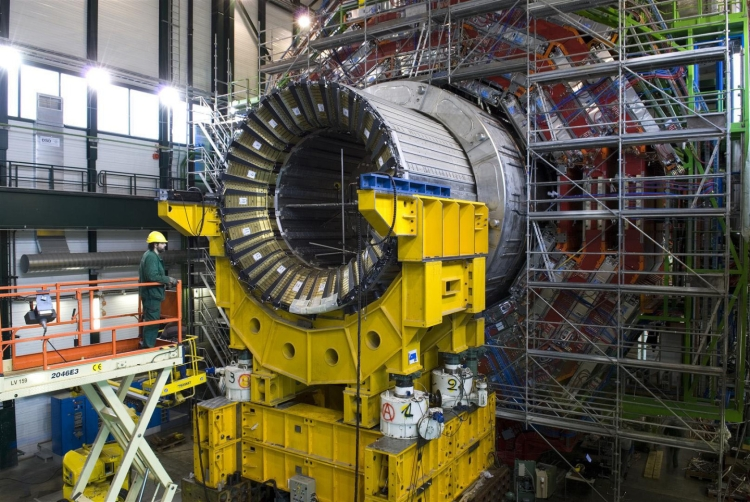
\includegraphics[width=0.8\textwidth,clip] {HCAL.jpg}
        \caption{Insertion of the HCAL barrel inside the magnet in 2008.}
        \label{fig:HCAL}
    \end{center}
\end{figure}

The HCAL is a sampling calorimeter meaning it finds a particle’s position, energy, and arrival time using alternating layers of dense ``absorber'' and fluorescent ``scintillator'' materials that produce a rapid light pulse when the particle passes through. Fitting the HCAL into the ``compact'' CMS required the use of very densely packed materials and geometry, since the minimum amount of material needed to contain and measure a hadron's shower is about one meter. 

To accomplish this feat, the HCAL is organised into barrel (HB and HO), endcap (HE), and forward (HF) sections. The endcaps are constructed from 36 ``wedges'' which measure particle energies as they emerge through the ends of the solenoid magnet. In addition, there are 36 barrel pieces, each weighing 26 tonnes, around the circumference of the barrel. These form the last layer of detectors inside CMS's magnet coil, since the outer barrel (HO) sits outside the coil to ensure that no energy escapes CMS undetected. 

Finally, the two hadronic forward calorimeters (HF) are positioned at either end of the detector, to capture any particles coming out of the collision region at large $\eta$, or shallow angles relative to the beam line. These receive the bulk of the energy from the particle collisions, so the HFs are very radiation hard.

\subsection{Muon System}

As its name suggests, detecting muons is one of the most important tasks of CMS. Muons are charged particles that are just like electrons and positrons, but 200 times heavier, and with much greater penetration depth. 
Because they can travel through several meters of material without losing much energy, unlike most created particles, they are not stopped by any of CMS calorimeters. Therefore, chambers specifically designed to detect muons are placed in the outer part of CMS, where they are likely to be the only particles producing a clear signal.



Muon hits are registered in the four muon stations, which are located outside of the magnet coil interleaved with the iron ``return yoke'' plates previously mentioned.

In total there are 1400 muon chambers: 250 drift tubes (DTs) and 540 cathode strip chambers (CSCs) track the particle positions and provide a trigger, while 610 resistive plate chambers (RPCs) and 72 gas electron multiplier chambers (GEMs) form a redundant trigger system, which quickly decides to keep or discard the acquired muon data. 


Muon tracking is achieved by measuring the curvature of muon trajectories in the $3.8\,\mathrm{T}$ magnetic field generated by the CMS solenoid.

The muon momentum is reconstructed by combining data from:
\begin{itemize}
	\item The muon chambers (for trajectory information).
	\item The silicon tracker (for high-precision tracking near the interaction point).
\end{itemize}
The combined resolution is approximately $3$--$5\%$ for transverse momentum $p_T > 10\,\mathrm{GeV/c}$.

The alignment of muon chambers is crucial for accurate tracking. Cosmic ray data and dedicated calibration runs are used to align the chambers to sub-millimeter precision.

Each detector type undergoes gas and electronic calibration to ensure timing and spatial measurements are accurate. This process includes:
\begin{itemize}
	\item Gas gain calibration for DT and CSC chambers.
	\item Timing calibration for RPC chambers.
\end{itemize}

\begin{itemize}
	\item The muon system achieves $>95\%$ detection efficiency for high-momentum muons.
	\item It integrates seamlessly with the calorimeters, inner tracker, and solenoid to provide a complete picture of collision events.
\end{itemize}

\subsubsection{Drift Tubes (DT)}
\begin{itemize}
	\item \textbf{Location:} DT chambers are located in the barrel region, covering a pseudorapidity range of $|\eta| < 1.2$.
	\item \textbf{Structure:} Each DT consists of parallel cylindrical drift tubes filled with a gas mixture, typically argon and carbon dioxide (CO$_2$).
	\item \textbf{Working Principle:} When a muon passes through a drift tube, it ionizes the gas. Electrons drift toward an anode wire under the influence of an electric field. The drift time provides precise position information.
	\item \textbf{Spatial Resolution:} Approximately $1$--$2\,\mathrm{mm}$.
	\item \textbf{Role:} DT chambers are used for both tracking and triggering, providing precise position and timing information.
\end{itemize}

\subsubsection{Cathode Strip Chambers (CSC)}
\begin{itemize}
	\item \textbf{Location:} CSCs are situated in the endcap regions, covering pseudorapidity ranges of $1.2 < |\eta| < 2.4$.
	\item \textbf{Structure:} Each CSC comprises multi-wire proportional chambers (MWPCs) with cathode strips for position readout.
	\item \textbf{Working Principle:} High-voltage differences between anode wires and cathode strips induce signals when muons pass through. Positions are reconstructed by measuring induced charge distributions.
	\item \textbf{Spatial Resolution:} Approximately $1\,\mathrm{mm}$ in the radial direction.
	\item \textbf{Role:} CSCs provide robust tracking in the forward region and contribute to the Level-1 (L1) trigger.
\end{itemize}

\subsubsection{Resistive Plate Chambers (RPC)}
\begin{itemize}
	\item \textbf{Location:} RPCs are deployed in both the barrel ($|\eta| < 1.6$) and endcap ($1.6 < |\eta| < 2.4$) regions.
	\item \textbf{Structure:} RPCs are made of resistive plates separated by a gas-filled gap. Typical gas mixtures include tetrafluoroethane (C$_2$H$_2$F$_4$) and sulfur hexafluoride (SF$_6$).
	\item \textbf{Working Principle:} Charged particles ionize the gas, creating avalanches that induce a fast signal across resistive plates.
	\item \textbf{Time Resolution:} Approximately $1\,\mathrm{ns}$.
	\item \textbf{Role:} RPCs provide fast timing information and are primarily used for triggering.
\end{itemize}


\begin{figure}
\centering
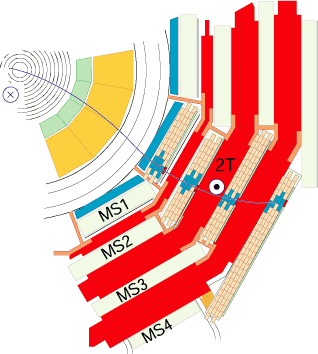
\includegraphics[width=0.80\textwidth]{figures/MuStations.png}
\caption{A muon, in the plane perpendicular to the LHC beams, leaves a curved trajectory in four layers of  muon ``stations.''}
\label{fig:MuStations}
\end{figure}    

\subsubsection{Muon Drift Tubes}

\begin{figure}
\centering
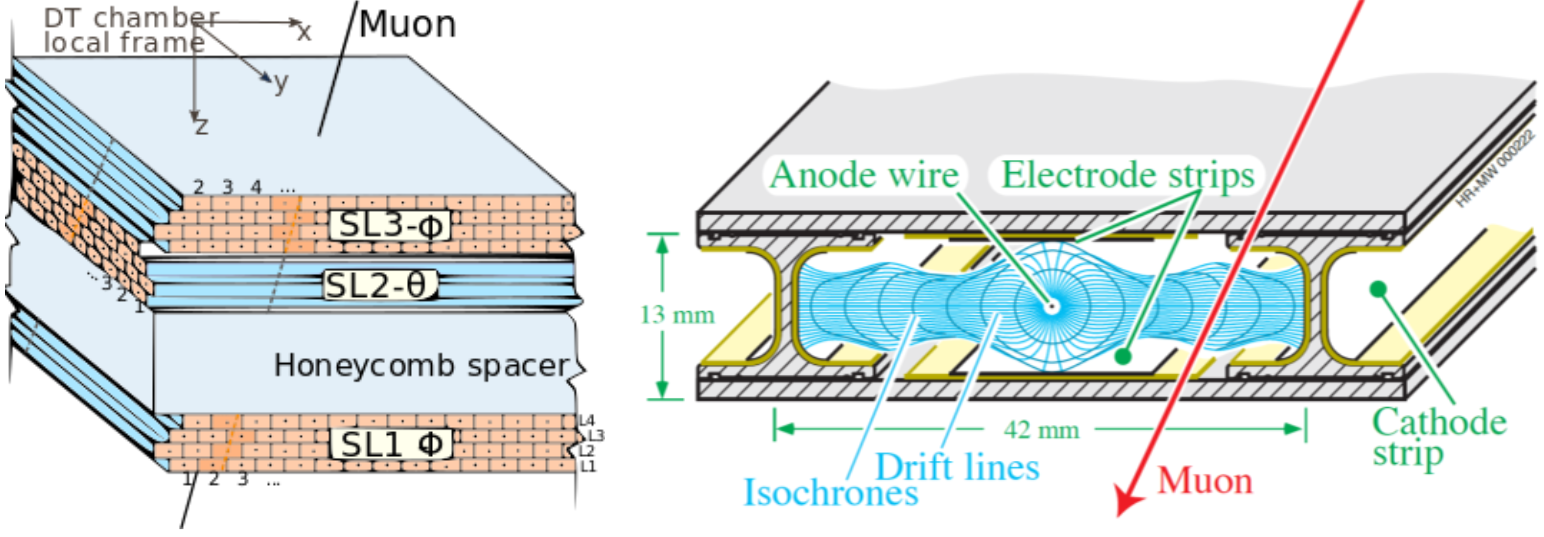
\includegraphics[width=0.80\textwidth]{figures/DTchambers.png}
\caption{The sizes of DT chambers range from  2m x 2.5m to 4m x 2.5m, approximately.}
\label{fig:DTchambers}
\end{figure}    

The drift tube (DT) system measures and identifies muon tracks in the barrel part of the detector. Each 4cm-wide tube contains a stretched wire within a gas volume. When a muon or any charged particle passes through the volume, it knocks electrons off the atoms of the gas. These electrons ``drift'' towards the anode following the electric field, ending up at the positively-charged wire where they are amplified and produce a measurable charge pulse. Each unit or ``superlayer'' contains four layers of staggered drift cells. By registering the time taken by the electrons to reach the wire, and since the drift velocity along the cell is a rather constant value, we can identify the exact crossing point of the muon along the cell.

\subsubsection{Cathode strip chambers}

\begin{figure}
\centering
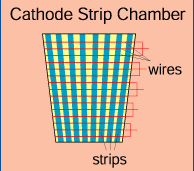
\includegraphics[width=0.80\textwidth]{figures/CSC.png}
\caption{}
\label{fig:CSC}
\end{figure}    

Cathode strip chambers (CSCs) are utilized in the endcap disks where the magnetic field is uneven, and particle rates are higher compared to the barrel. The chambers are made up of arrays of positively-charged anode wires intersecting with negatively-charged copper cathode strips within a gas-filled chamber. 

When muons pass through the chamber, they ionize the gas atoms, causing electrons to be knocked free. These electrons are attracted to the anode wires, creating an avalanche effect. Meanwhile, the positive ions move away from the wires and toward the copper cathode strips, generating a charge pulse in the strips, which occurs at a right angle to the direction of the wires. Since the wires run perpendicular to the strips, we get two position coordinates for each passing particle.

\subsubsection{Resistive Plate Chambers}

\begin{figure}
\centering
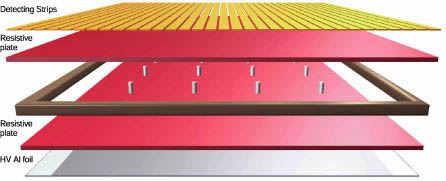
\includegraphics[width=0.80\textwidth]{figures/RPClayers.jpg}
\caption{}
\label{fig:RPClayers}
\end{figure}

Resistive Plate Chambers (RPCs) are fast gaseous detectors that provide a muon trigger system, consisting of two parallel plates acting as an anode and cathode. The plates are both made of a very high resistivity plastic material and separated by a thin gas volume.

\subsubsection{Gas Electron Multipliers}

\begin{figure}
\centering
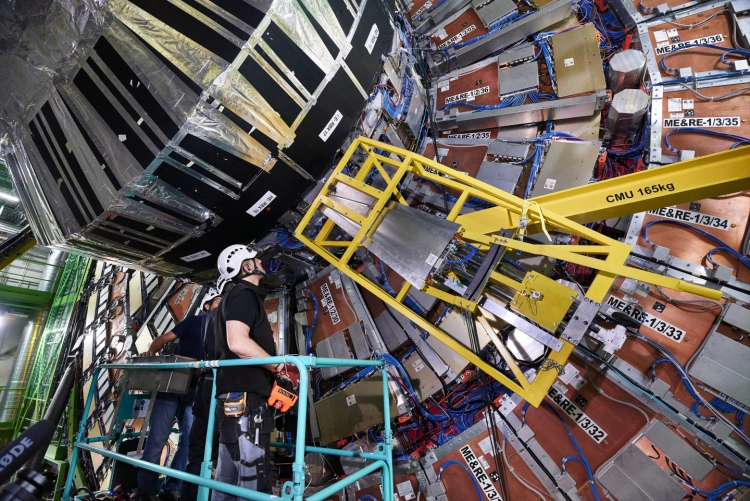
\includegraphics[width=0.80\textwidth]{figures/GEMinstallation.jpg}
\caption{Gas Electron Multiplier chamber installation.}
\label{fig:GEMinstallation}
\end{figure}

Gas electron multipliers (GEMs) are a new addition to the CMS muon system. They complement existing detectors in the forward regions close to the beampipe, where large radiation doses and high event rates will increase during Phase-2 of the LHC.

Like the other CMS muon subsystems, GEMs are gaseous detectors. Their key feature is the GEM foil, which consists of a 50 micrometer-thick insulating polymer (polyimide) surrounded on the top and bottom with copper conductors. Throughout the foil, microscopic holes are etched in a regular hexagonal pattern. The CMS GEM chambers consist of two PCBs, containing the gas volume, and a stack of three GEM foils in between. The chambers are filled with an Ar/CO2 gas mixture, which is ionized by incident ionizing particles. A potential difference applied across the foils generates sharp electric fields in the holes. The electrons created during the ionisation process drift towards the foils and are multiplied in the holes. The resulting electron avalanche induces a readout signal on the finely spaced strips.

\section{Triggers and Data Acquisition System}

Level 1 of the trigger is an extremely fast and wholly automatic process that looks for simple signs of interesting physics, e.g. particles with a large amount of energy or in unusual combinations.

One consequence of the decision was that L1 has to be more efficient than in previous systems in order to perform certain tasks traditionally performed by L2.

The muon chambers contribute significantly to the CMS trigger system, which is essential for selecting interesting collision events in real-time.

\subsection{Level-1 Trigger}
The L1 trigger uses coarse information from the DT, CSC, and RPC subsystems to identify high-transverse-momentum ($p_T$) muons. It operates within a latency of a few microseconds.

\subsection{High-Level Trigger (HLT)}
The HLT refines L1 trigger candidates by combining muon chamber data with inner tracker information. This process involves more sophisticated algorithms for precise momentum reconstruction.




\section{Computing}

Even with the triggers reducing the amount of unnecessary data coming out of our detector, CMS still produces a huge amount of data that must be analysed -- more than 5 Pb per year when running at peak performance.

The ``Tier 0'' center at CERN is the first to reconstruct full collision events, where analysts begin searching for patterns in the data. 
Then, after CERN creates a primary backup, the data is sent to large ``Tier 1'' computer centers located in seven different countries: France, Germany, Italy, Spain, Taiwan, the UK, and the US. 
At these centers, the events are reconstructed again, with improved calculations using refined calibration constants based on experimental information.

Tier 1 centers begin to interpret and analyze the particle events, compiling the results to identify emerging patterns. Simultaneously, each Tier 1 center sends the most complex events to a network of around 40 ``Tier 2'' facilities for further specialized analysis. This tiered system efficienty processes all CMS data while also allowing information to be distributed globally, regularly updated by the LHC Computing Grid.

\section{Particle Reconstruction}

The Particle Flow (PF) algorithm aims at reconstructing and identifying all stable particles in the event with a thorough combination of all CMS sub-detectors towards an optimal determination of their direction, energy and type. This list of individual particles is then used, as if it came from a Monte-Carlo event generator, to build jets (from which the quark and gluon energies and directions are inferred), to determine the missing transverse energy (which gives an estimate of the direction and energy of the neutrinos and other invisible particles), to reconstruct and identify particles from their decay products, and more \cite{Beaudette:1645993}.

\section{Alignment of the CMS Tracker}

\subsection{Parameterization}

\begin{figure}[!htb]
    \begin{center}
        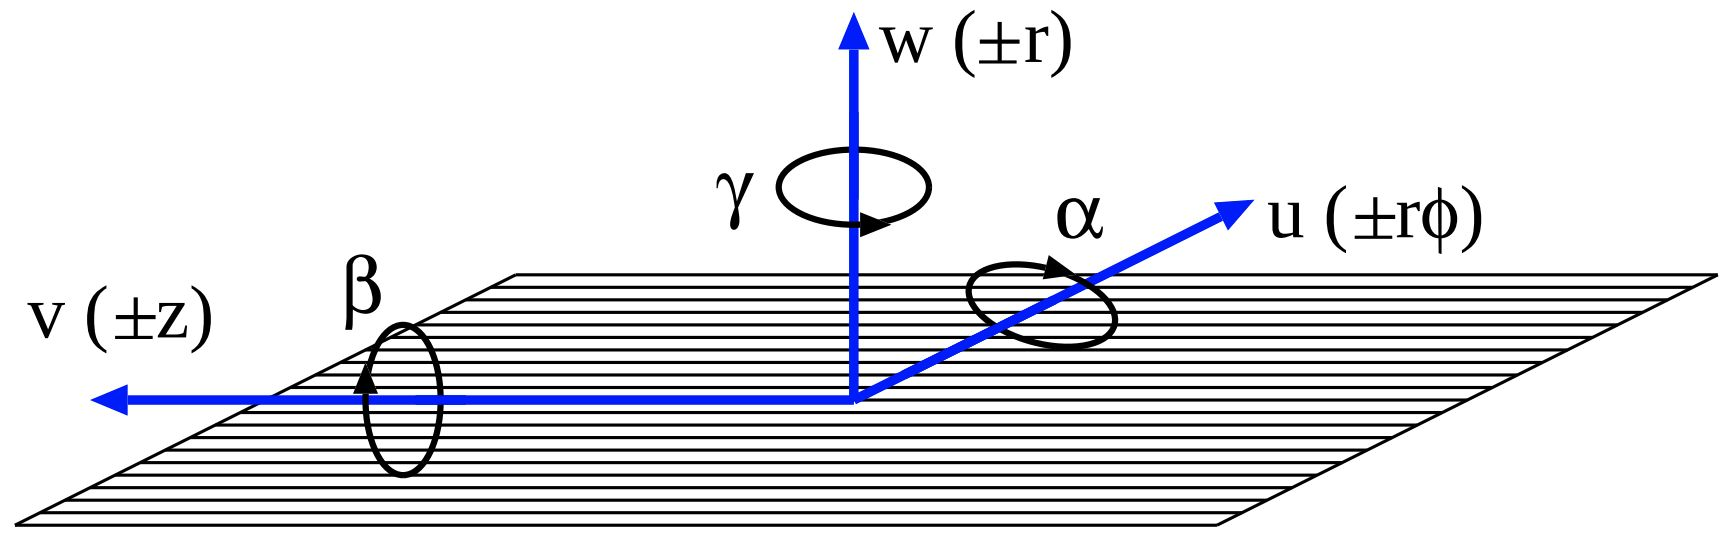
\includegraphics[width=0.8\textwidth,clip] {TrackerParam.jpg}
        \caption{Example local coordinates of a module. Global parameters are shown in parentheses for modules in the TIB and TOB \cite{WAdam_2009}.}
        \label{fig:TrackerParam}
    \end{center}
\end{figure}

Hit positions and impact points of a track are systematically displaced if the module position is not known correctly.

The difference in local module coordinates between these two quantities are the ``track-hit residuals'' \cite{Karimaki:926537}.

Modules are parameterized as seen in Fig.~\ref{fig:overlapHits}:
\begin{itemize}
    \item w axis is normal to the module
    \item u and v axes are in the plane
    \item u axis more sensitive to direction of measurement
    \item Angles $\alpha$, $\beta$, and $\gamma$ describe rotations around u, v, w respectively
\end{itemize}

Hierarchical systems:
\begin{itemize}
    \item \{r, g, q\} = coordinates in \{global, composite, local\} system
    \item \{R, G\} = rotations between global and \{local, composite\} system
\end{itemize}

\begin{figure}[!htb]
    \begin{center}
        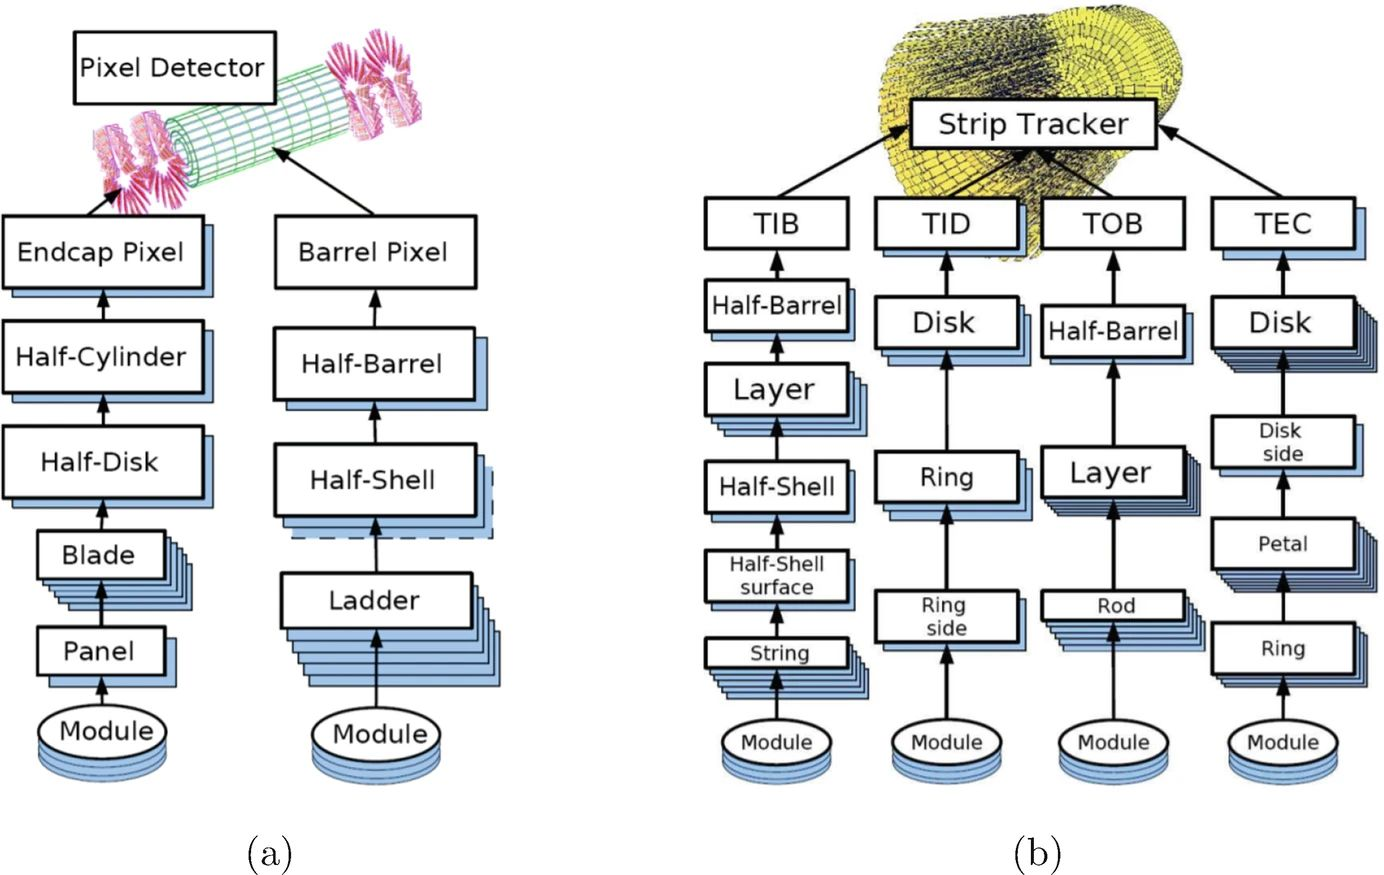
\includegraphics[width=0.8\textwidth,clip] {HLS.jpg}
        \caption{Diagrams of the hierarchical structures of the Pixel Detector and Strip Tracker \cite{WAdam_2009}.}
        \label{fig:HLS}
    \end{center}
\end{figure}

\subsection{Algorithms}

\begin{figure}[!htb]
    \begin{center}
        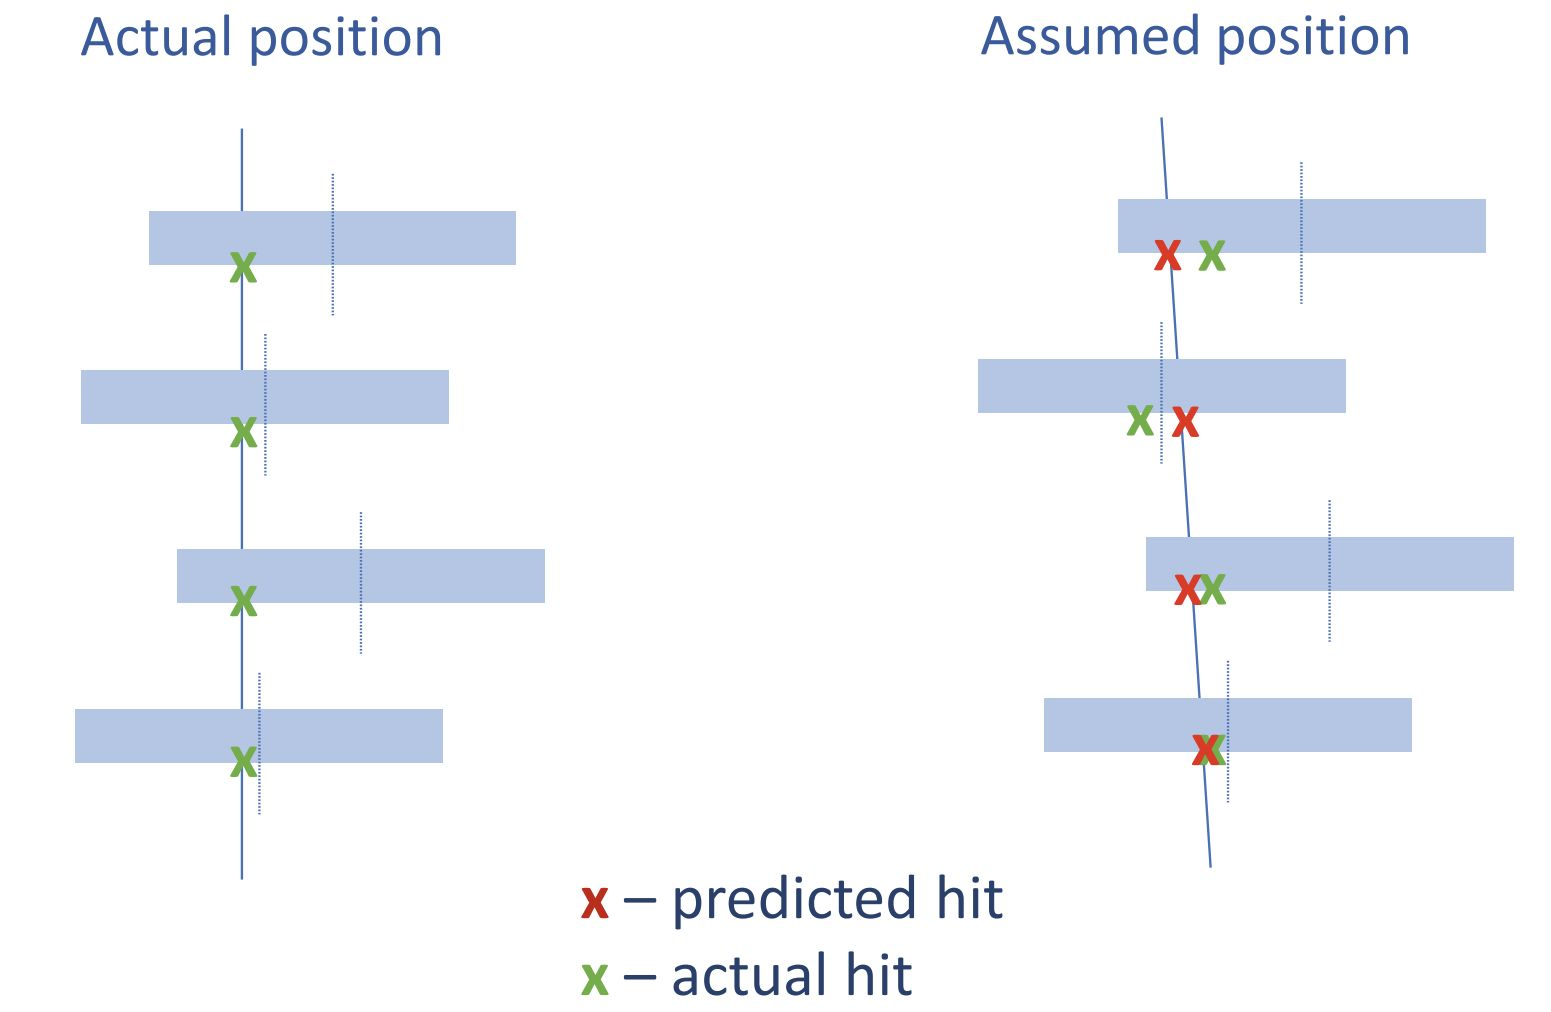
\includegraphics[width=0.8\textwidth,clip] {overlapHits.jpg}
        \caption{Simple illustration of a track through misaligned layers \cite{2022166795}.}
        \label{fig:overlapHits}
    \end{center}
\end{figure}

\subsubsection{MillePede}

% \begin{figure}[!htb]
%     \begin{center}
%         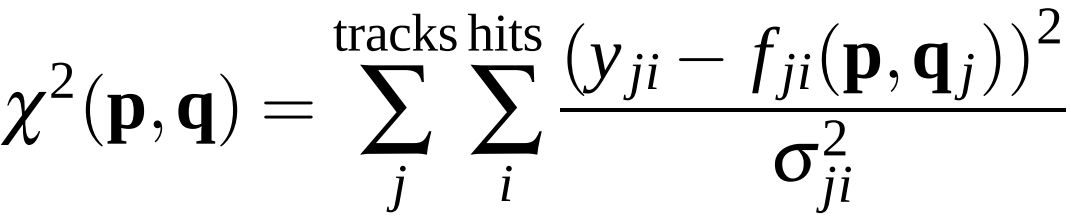
\includegraphics[width=0.8\textwidth,clip] {chi2MPiteration.jpg}
%         \caption{$\Xi^2$ function for MILLEPEDE-II global fit \cite{WAdam_2009}.}
%         \label{fig:chi2MPiteration}
%     \end{center}
% \end{figure}

\begin{equation}
\label{eq:MPX2}
\begin{gathered}
\mathcal{X} ^2 (p, q) = \Sigma_j^{tracks} \Sigma_i^{hits} \frac{(y_{ji} - f_{ji}(p, q_j))^2}{\sigma_{ji}^2}
\end{gathered}
\end{equation}

Unlike HipPy, MILLEPEDE-II (MP) opts to use a global matrix and forgoes the iterative approach.

\subsubsection{HipPy}

\begin{figure}[!htb]
    \begin{center}
        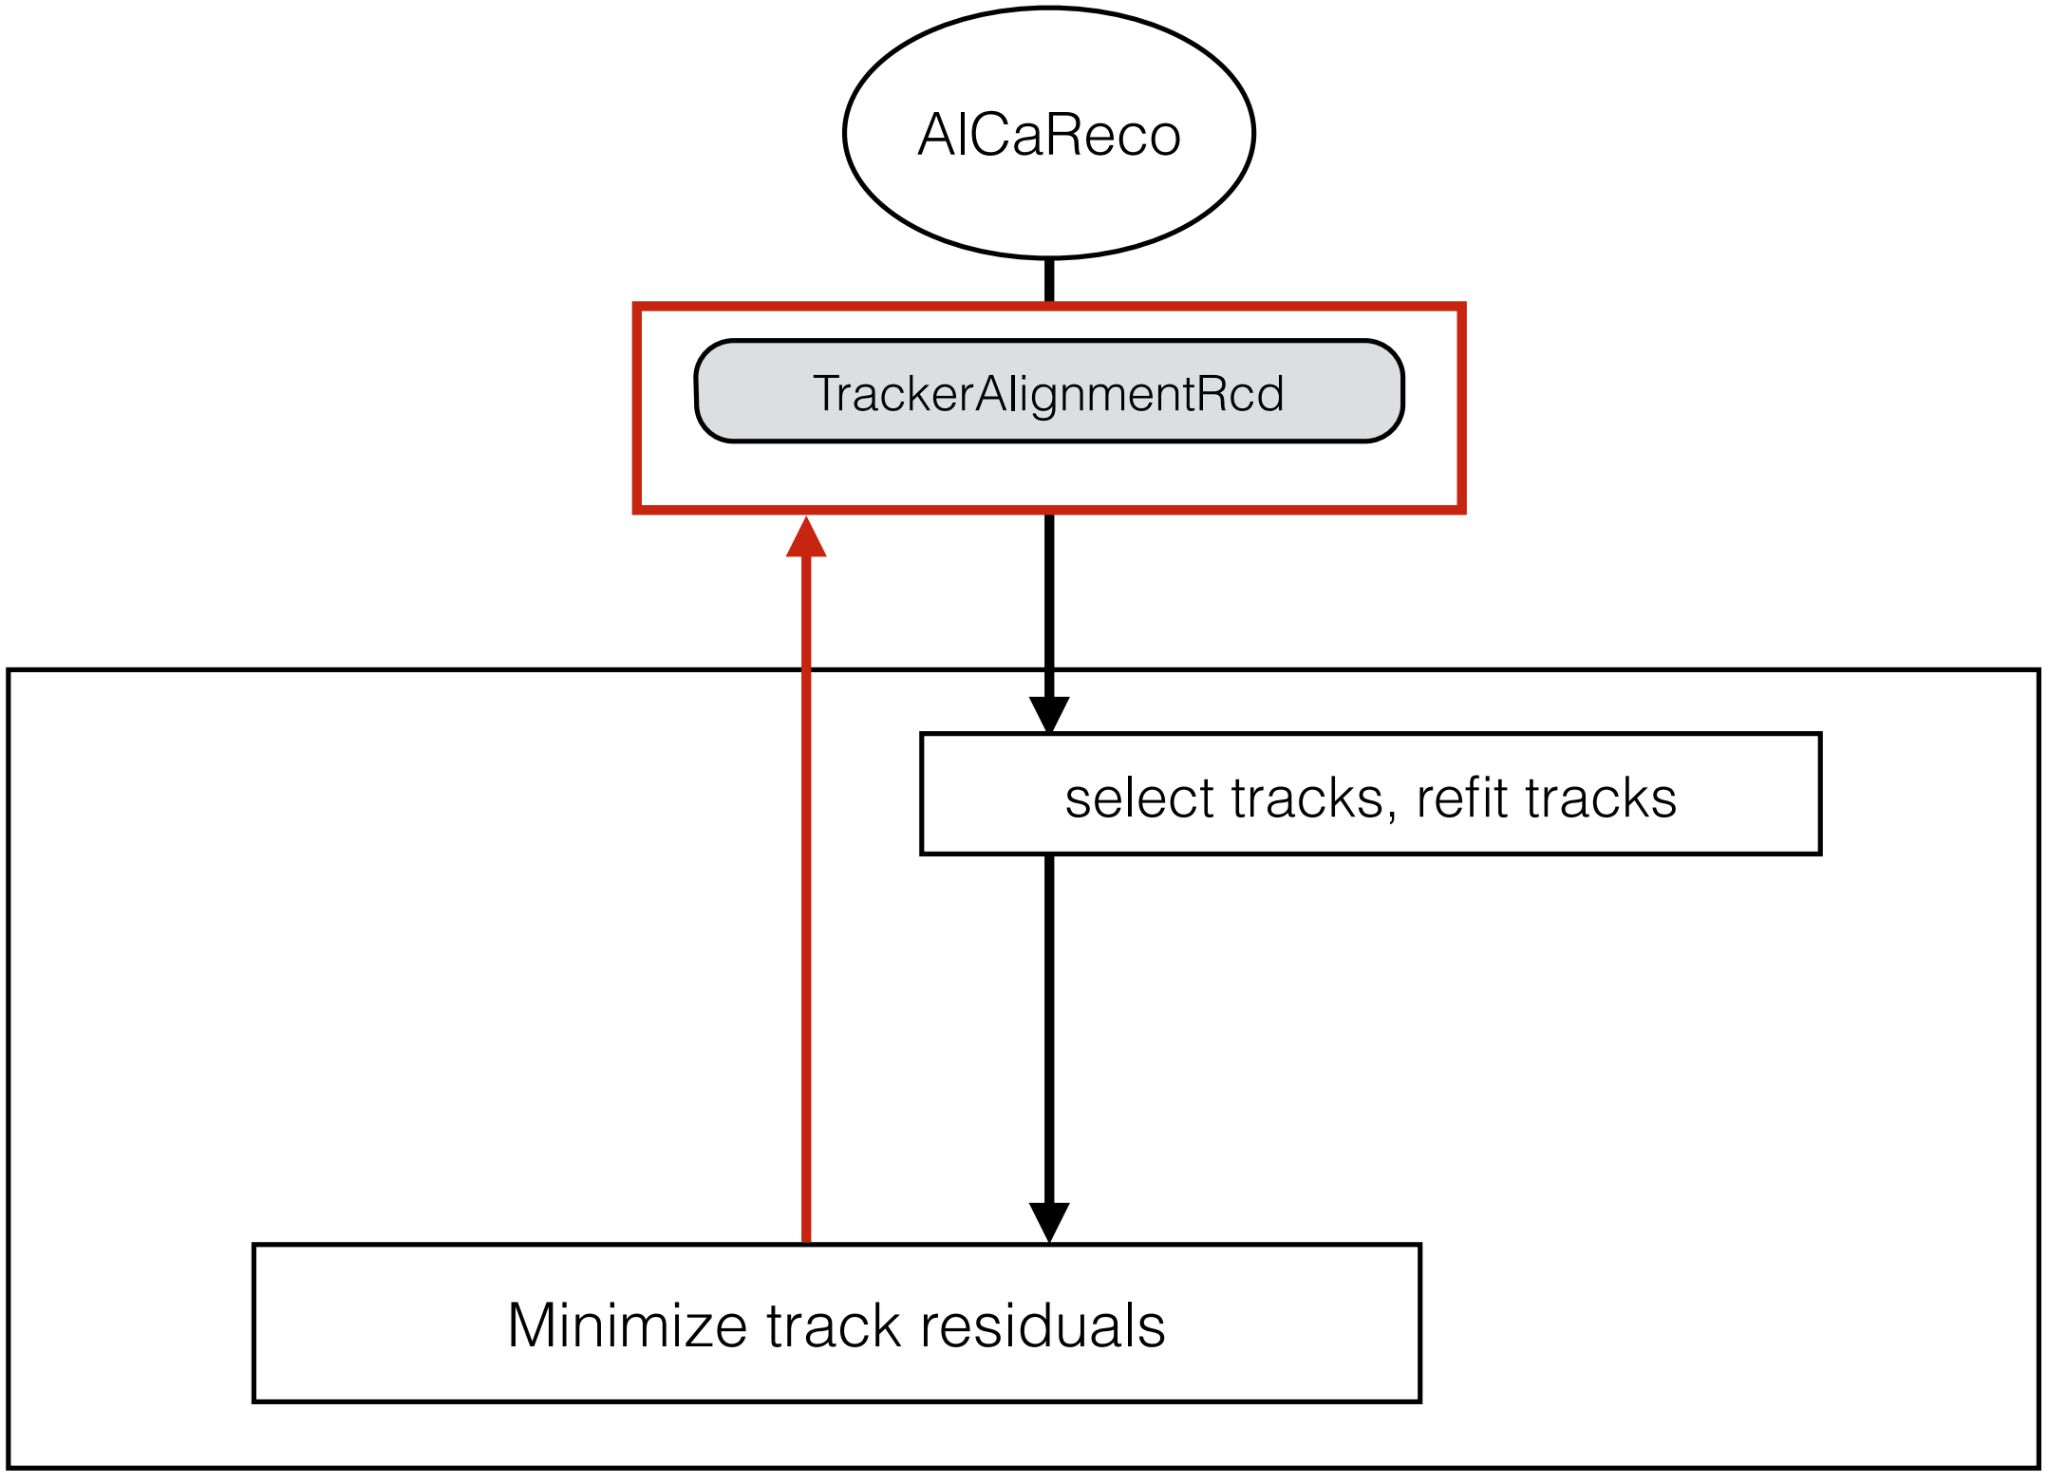
\includegraphics[width=0.8\textwidth,clip] {HIP.jpg}
        \caption{Process diagram of the Hits-and-Impact-Points (HIP) alignment algorithm \cite{2022166795}.}
        \label{fig:HIP}
    \end{center}
\end{figure}

\begin{figure}[!htb]
    \begin{center}
        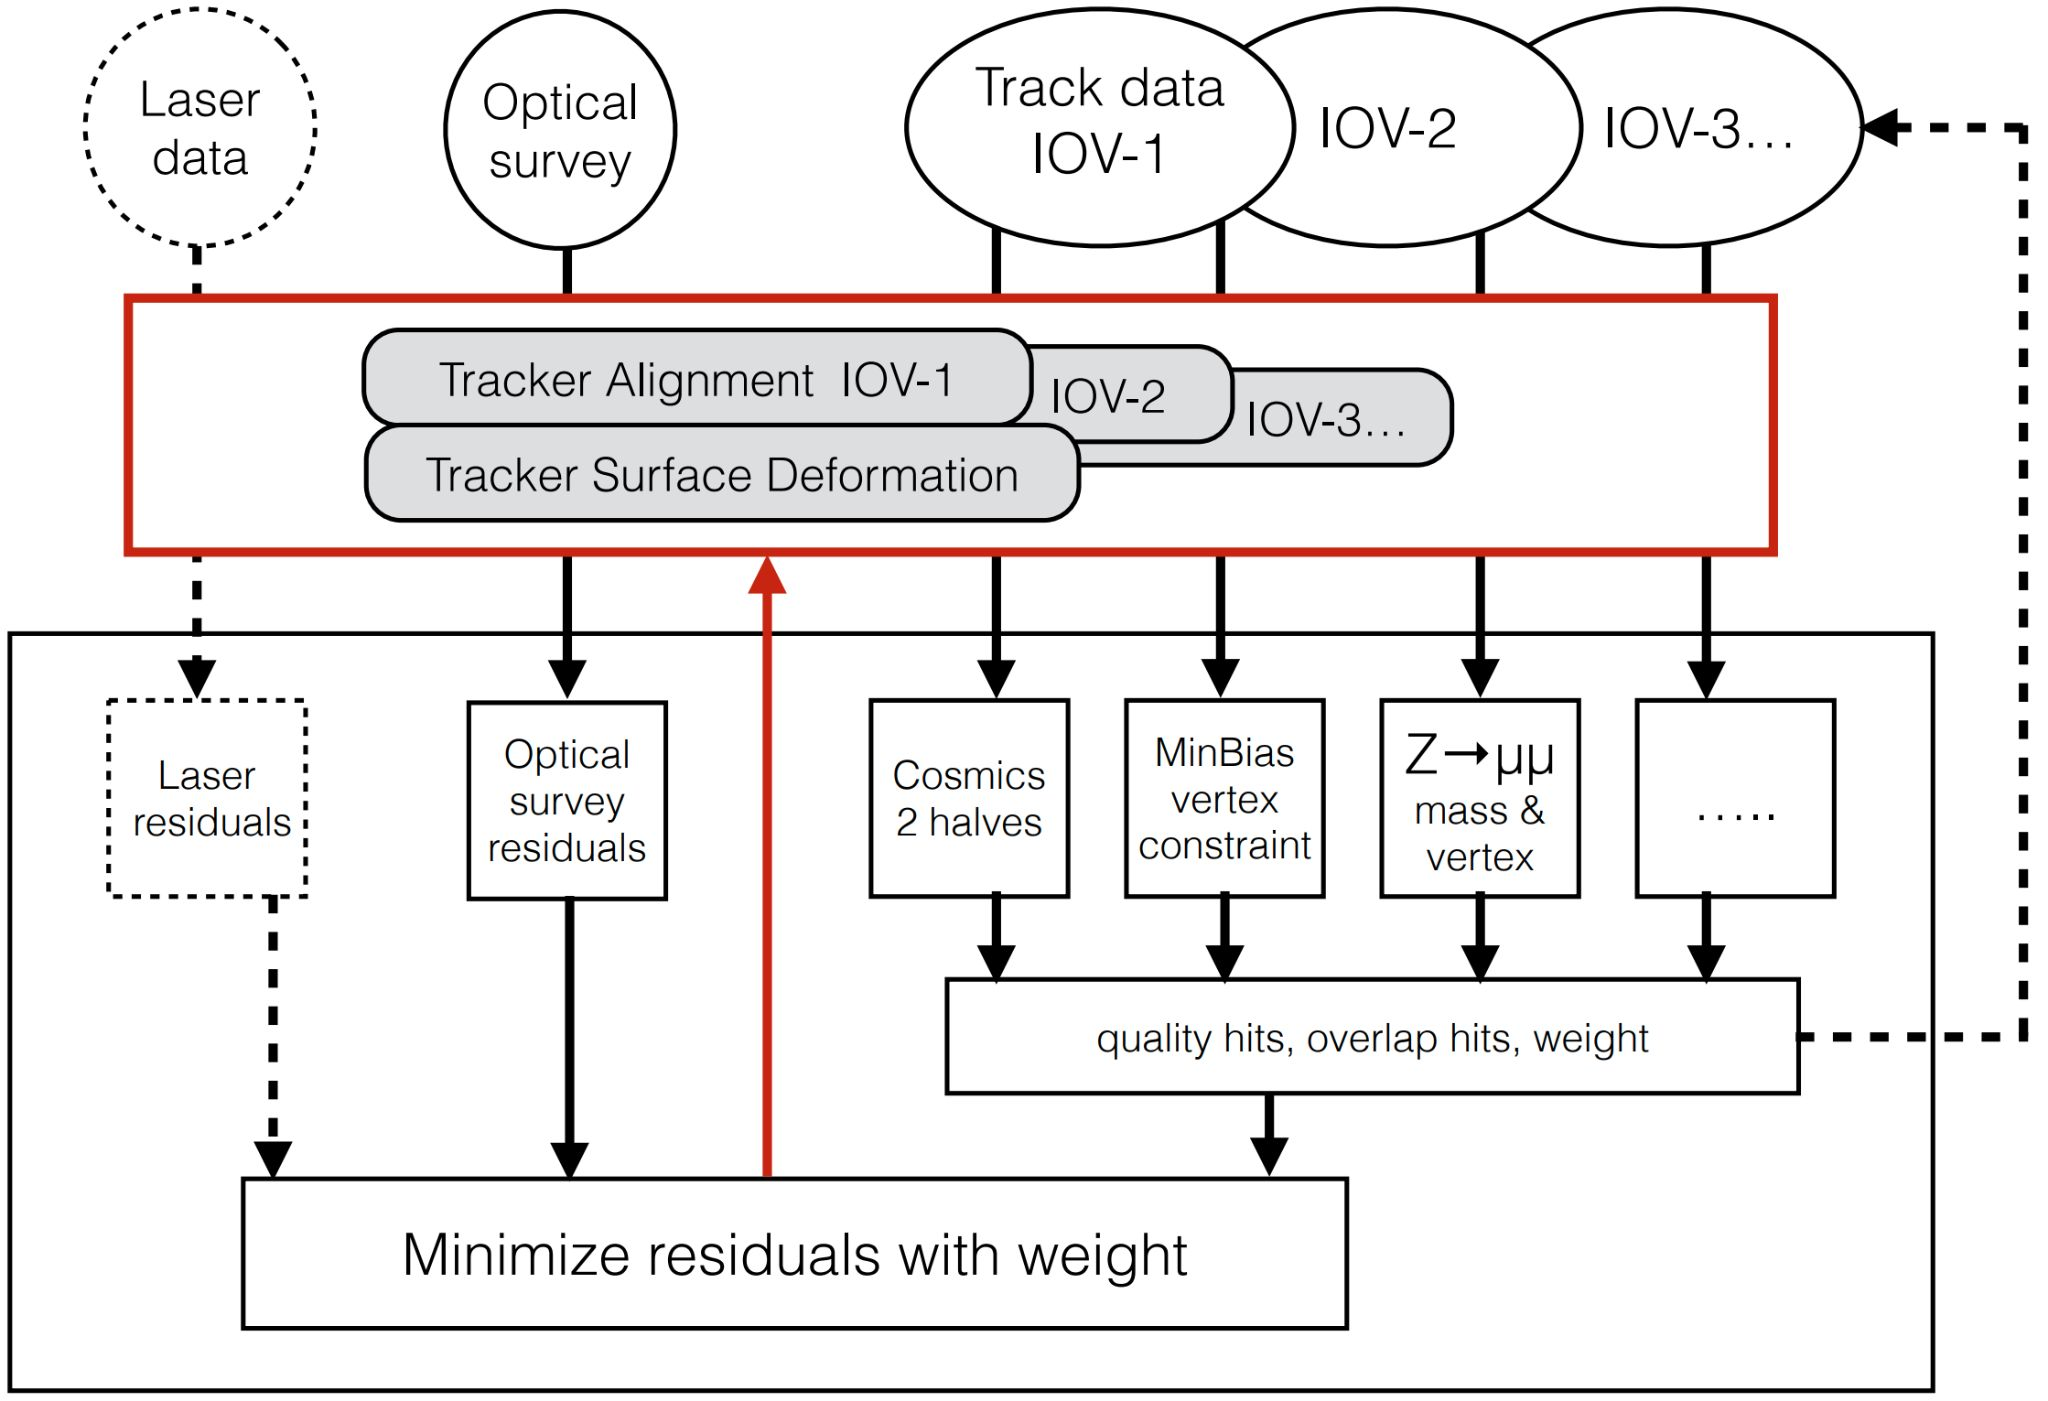
\includegraphics[width=0.8\textwidth,clip] {HipPy.jpg}
        \caption{Process diagram of the Hits-and-Impact-Points-Past-Year-1 (HipPy) alignment algorithm \cite{2022166795}.}
        \label{fig:HipPy}
    \end{center}
\end{figure}

% \begin{figure}[!htb]
%     \begin{center}
%         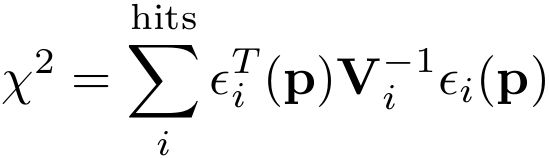
\includegraphics[width=0.8\textwidth,clip] {chi2HPiteration.jpg}
%         \caption{$\Xi^2$ function for HipPy fit.}
%         \label{fig:chi2HPiteration}
%     \end{center}
% \end{figure}

% \begin{figure}[!htb]
%     \begin{center}
%         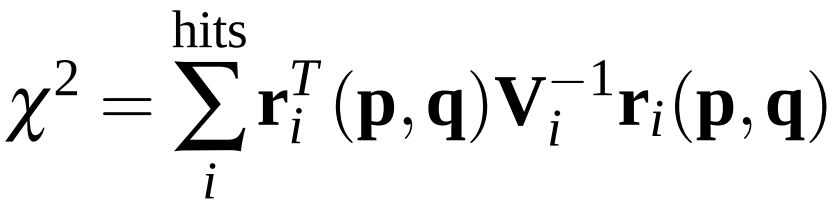
\includegraphics[width=0.8\textwidth,clip] {chi2HPiteration2.jpg}
%         \caption{$\Xi^2$ function for HipPy fit.}
%         \label{fig:chi2HPiteration2}
%     \end{center}
% \end{figure}

% \begin{figure}[!htb]
%     \begin{center}
%         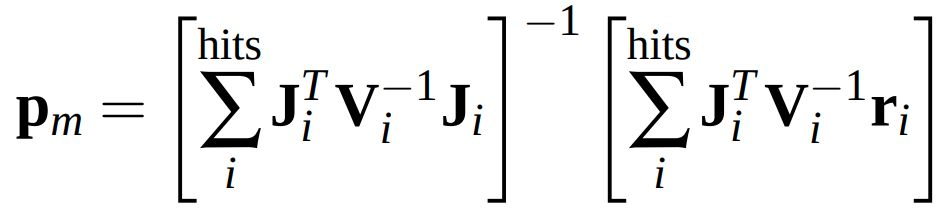
\includegraphics[width=0.8\textwidth,clip] {pmHPiteration.jpg}
%         \caption{Alignment parameters $p_m$ for HipPy fit.}
%         \label{fig:pmHPiteration}
%     \end{center}
% \end{figure}

The ``hits-and-impact-points'' (HIP) algorithm \cite{Karimaki:2003bd,Karimaki:926537} precedes what we now call HipPy.
Utilized during commissioning \cite{WAdam_2009} of the CMS tracker and for Run 1 \cite{CMSCollaboration_2010,Chatrchyan:1667597}.

Several notable features were added over time \cite{BROWN2009467} and the improved algorithm was renamed to “hits-and-impact-points-past-year-1” (HipPy) at the start of Run 2. 

Improvements to the alignment algorithm since Run 1:
\begin{itemize}
    \item The inclusion of 3 alignment parameters to describe sensor curvature (beyond the 6 position/orientation coordinates)
    \item The ability to weight certain types of input
    \item The option to perform sequential, hierarchical alignment over multiple time periods (multi-IOV)
    \item Optional mass and/or vertex constraints in certain types of events with known physics process
\end{itemize}

These features proved invaluable during Run 2, with successful HipPy-based alignment constants used in CMS data reconstruction (along with MP objects) in the prompt and EOY alignments\cite{BROWN2009467}.

The basic outline of the hits-and-impact-points (HIP) algorithm is as follows \cite{BROWN2009467}:
\begin{itemize}
    \item Load track data and hits
    \item The tracks are fit using the current estimate of the alignment parameters
    \item Hit $\mathcal{X} ^2$ are computed for the selected hits, following the definition in Eq.~\ref{eq:HIPX2}
    \item Minimize each sensor’s $\mathcal{X} ^2$ w.r.t. a change in only that sensor’s local alignment
    \item Hold the parameters of every other sensor fixed
    \item Calculate for every sensor
    \item Update the alignment parameters for all sensors with the computed change to the original estimate
    \item Use the updated local alignment to fit the tracks for the next iteration
    \item Repeat the process until the alignment converges
\end{itemize}

\begin{equation}
\label{eq:HIPX2}
\begin{gathered}
\mathcal{X} ^2 = \Sigma_i^{hits} \epsilon_i^T(p) V^{-1}_i \epsilon_i(p)
\end{gathered}
\end{equation}

\begin{itemize}
    \item HipPy leverages full integration of CMS software, which is helpful especially for track reconstruction
    \item Can make use of any constraint (e.g. mass, vertex) defined in that software
    \item Adds flexibility and simplifies development (e.g. Kalman filter)
    \item Position and orientation of each sensor are determined independently of other sensors in every iteration
    \item Multiple iterations are required to solve correlations between sensor parameters (requires multiple track fits)
    \item But each iteration is a straightforward application of a small matrix inversion
\end{itemize}

\begin{equation}
\label{eq:HPX2}
\begin{gathered}
\mathcal{X} ^2 = \Sigma_i^{hits} r_i^T(p, q) V^{-1}_i r_i(p, q)
\end{gathered}
\end{equation}

\begin{equation}
\label{eq:HPpm}
\begin{gathered}
p_m = [\Sigma_i^{hits} J^T_i V^{-1}_i J_i]^{-1} [\Sigma_i^{hits} J^T_i V^{-1}_i r_i]
\end{gathered}
\end{equation}

\begin{figure}[!htb]
    \begin{center}
        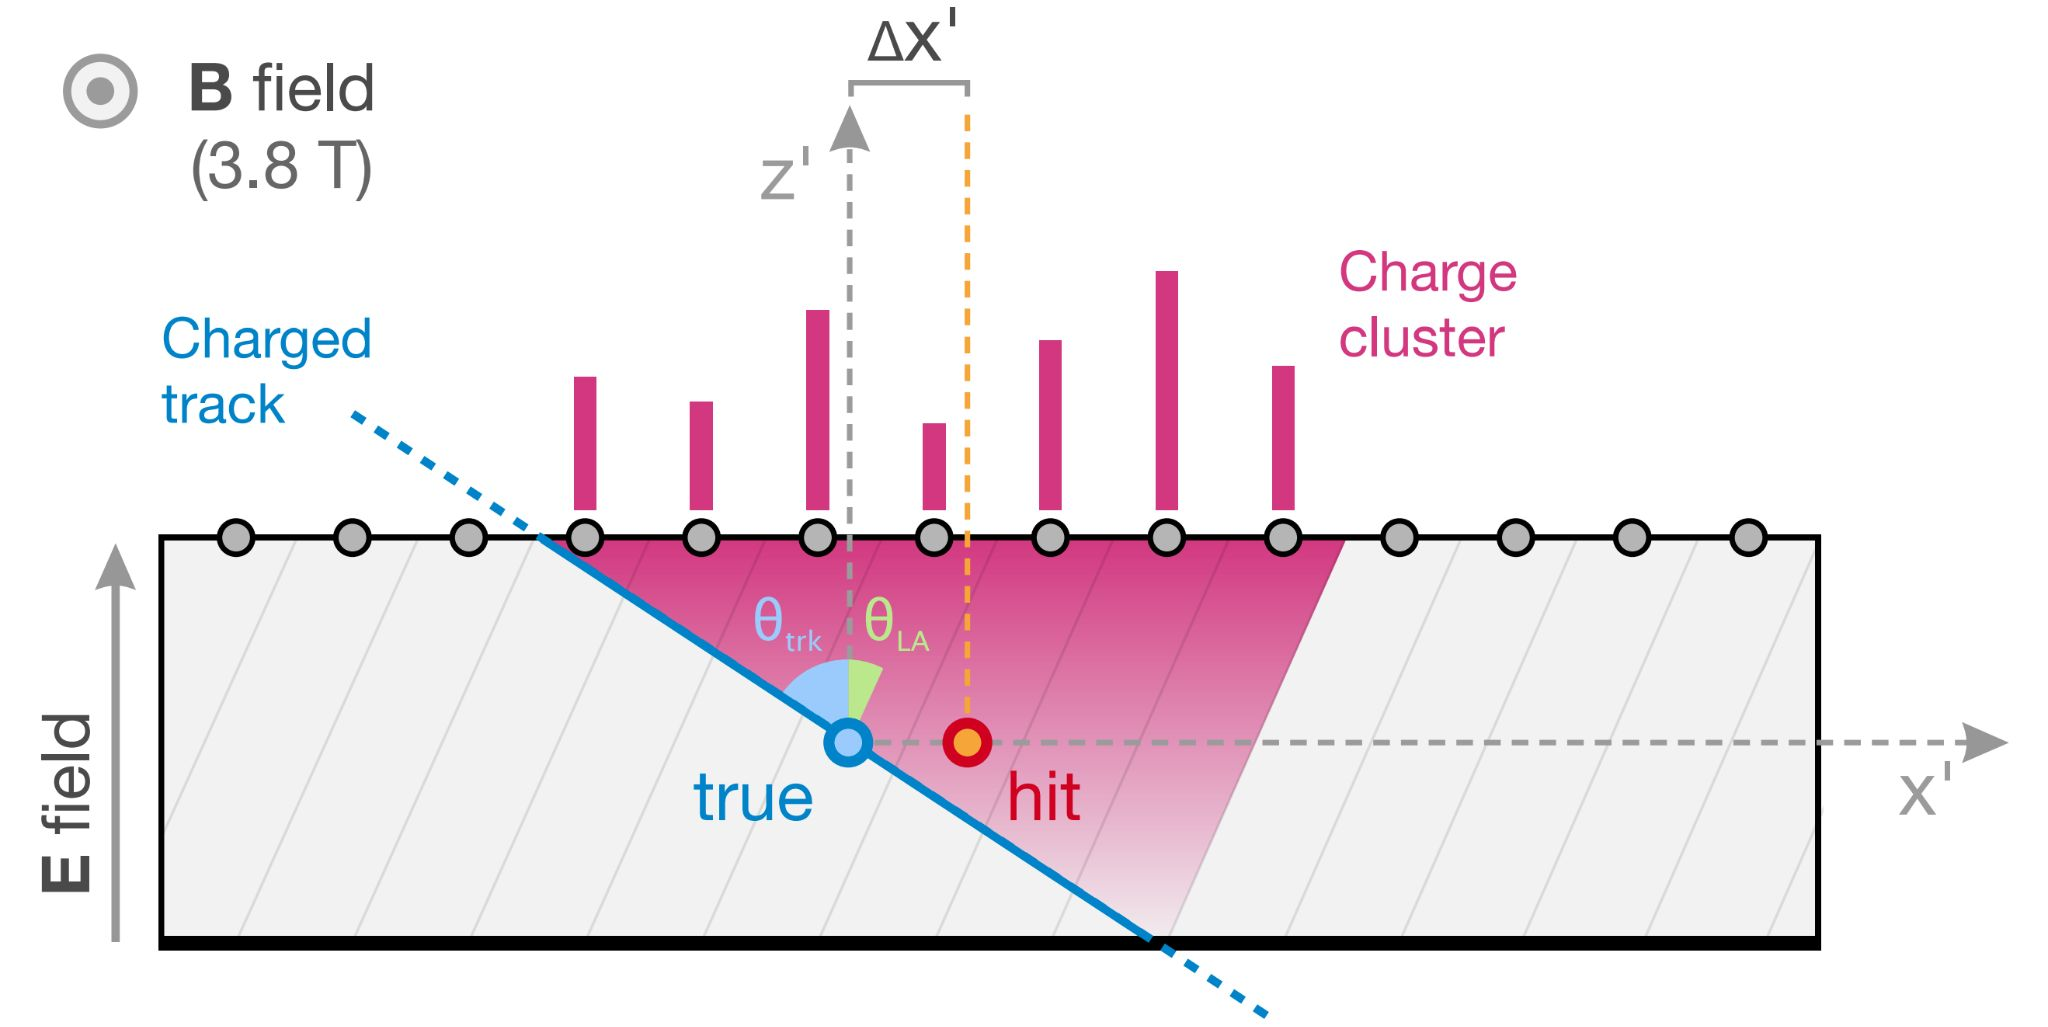
\includegraphics[width=0.8\textwidth,clip] {siliconmodule.jpg}
        \caption{Transverse view of a silicon module \cite{2022166795}.}
        \label{fig:siliconmodule}
    \end{center}
\end{figure}



\subsection{Validation}


\subsubsection{Geometry Comparison}


\subsubsection{Distribution of Median Residuals}


\subsubsection{Primary Vertex}


\subsubsection{Cosmic Track Splitting}


\subsubsection{Dimuon Validation}

$Z \rightarrow \mu\mu$

